\documentclass[12pt,a4paper]{article}

% ---Packages -----------------------------------------------------------------
\usepackage[utf8]{inputenc}
\usepackage[T1]{fontenc}
\usepackage[english]{babel}
\usepackage{geometry}
\usepackage{graphicx}
\usepackage{listings}
\usepackage{xcolor}
\usepackage{amsmath}
\usepackage{amssymb}
\usepackage{hyperref}
\usepackage{indentfirst}
\usepackage{booktabs}
\usepackage{array}
\usepackage{caption}
\usepackage{subcaption}
\setlength{\parindent}{1.25cm}

\geometry{a4paper, left=2.5cm, right=2cm, top=2cm, bottom=2cm}

\hypersetup{colorlinks=true, linkcolor=blue!60!black, urlcolor=blue!60!black}

\lstdefinestyle{pythonstyle}{
	language=Python,
	basicstyle=\ttfamily\small,
	keywordstyle=\color{blue!80!black}\bfseries,
	commentstyle=\color{green!55!black}\itshape,
	stringstyle=\color{orange!80!black},
	numbers=left,
	numberstyle=\tiny\color{gray},
	stepnumber=1,
	numbersep=8pt,
	backgroundcolor=\color{gray!8},
	showspaces=false,
	showstringspaces=false,
	showtabs=false,
	frame=single,
	rulecolor=\color{gray!40},
	tabsize=4,
	captionpos=b,
	breaklines=true,
	breakatwhitespace=false,
	xleftmargin=10pt,
	xrightmargin=5pt
}
\lstset{style=pythonstyle}

% -----------------------------------------------------------------------------
\begin{document}
	
	% ---Title page ----------------------------------------------------------------
	\begin{titlepage}
		\centering
		\vspace*{1cm}
		{\Large Ministerul Educa\c{t}iei \c{s}i Cercet\u{a}rii al Republicii Moldova\\}
		\vspace{0.5cm}
		{\Large Universitatea Tehnic\u{a} a Moldovei\\}
		\vspace{0.3cm}
		{\Large Facultatea Calculatoare, Informatic\u{a} \c{s}i Microelectronic\u{a}\\}
		\vspace{3cm}
		{\LARGE\bfseries Laboratory Work No.~3:\\}
		\vspace{0.5cm}
		{\LARGE\bfseries Study and Empirical Analysis\\}
		\vspace{0.3cm}
		{\LARGE\bfseries of Graph Traversal Algorithms:\\}
		\vspace{0.3cm}
		{\LARGE\bfseries BFS and DFS\\}
		\vspace{4cm}
		\begin{flushleft}
			\hspace{6cm}Elaborated: st. gr. FAF-241 Lungu Ilie\\
			\vspace{1cm}
			\hspace{6cm}Verified: asist. univ. Fistic Cristofor\\
		\end{flushleft}
		\vfill
		{\large Chi\c{s}in\u{a}u -- 2026}
	\end{titlepage}
	
	\newpage
	\tableofcontents
	\newpage
	
	% -----------------------------------------------------------------------------
	\section{OBJECTIVE}
	% -----------------------------------------------------------------------------
	
	The subject of this laboratory work is the study and empirical analysis of two
	fundamental graph traversal algorithms: \textbf{Breadth-First Search (BFS)} and
	\textbf{Depth-First Search (DFS)}. For each algorithm both an \emph{original} and
	an \emph{optimized} implementation are provided, and their performance is compared
	empirically across graphs of varying sizes. Visual diagrams are included to
	illustrate how each algorithm traverses a graph step-by-step. All implementations
	are written in pure Python so that execution times reflect genuine algorithmic
	differences rather than disparities between compiled and interpreted code.
	
	% -----------------------------------------------------------------------------
	\section{TASK 1 -- ALGORITHM IMPLEMENTATION}
	% -----------------------------------------------------------------------------
	
	\subsection{Complexity Reference}
	
	Table~\ref{tab:complexity} summarises the theoretical time and space complexity
	of both algorithms used as the baseline for interpreting the empirical results.
	$V$ denotes the number of vertices and $E$ the number of edges.
	
	\begin{table}[h!]
		\centering
		\caption{Theoretical complexity of BFS and DFS.}
		\label{tab:complexity}
		\renewcommand{\arraystretch}{1.3}
		\begin{tabular}{lcccc}
			\toprule
			\textbf{Algorithm} & \textbf{Time Complexity} & \textbf{Space Complexity} & \textbf{Shortest Path} & \textbf{Graph Type} \\
			\midrule
			BFS & $O(V + E)$ & $O(V)$ & Yes (unweighted) & Any \\
			DFS & $O(V + E)$ & $O(V)$ & No               & Any \\
			\bottomrule
		\end{tabular}
	\end{table}
	
	% ---1.1 BFS -------------------------------------------------------------------
	\subsection{Breadth-First Search (BFS)}
	
	\subsubsection{How It Works}
	
	BFS explores a graph \emph{level by level}, starting from a source node. It uses
	a queue (FIFO) to maintain the frontier of nodes yet to be visited. All immediate
	neighbours of the current node are enqueued before any of their children are
	explored, guaranteeing that nodes are visited in non-decreasing order of their
	hop-distance from the source. This property makes BFS the canonical algorithm for
	finding shortest paths in unweighted graphs.
	Figure~\ref{fig:viz_bfs} illustrates the level-by-level expansion on a small graph.
	
	\begin{figure}[h!]
		\centering
		\includegraphics[width=0.88\textwidth]{viz_bfs.png}
		\caption{BFS level-by-level traversal on a ten-node undirected graph.
			Nodes are coloured by the order in which they are first reached;
			dashed rings delimit each successive frontier level.}
		\label{fig:viz_bfs}
	\end{figure}
	
	\subsubsection{Original Implementation}
	
	The original BFS uses Python's \texttt{collections.deque} as the queue.
	Neighbours are appended to the right and consumed from the left, maintaining
	FIFO order.  A \texttt{set} tracks visited nodes to avoid revisiting any node on
	graphs with cycles.  Time complexity is $O(V+E)$; auxiliary space is $O(V)$ for
	the visited set and queue.
	
	\begin{lstlisting}[caption={BFS (original) -- queue-based level-order traversal.}]
from collections import deque
		
def bfs(graph, start):
	visited = set()
	queue   = deque([start])
	visited.add(start)
	order   = []
	while queue:
		node = queue.popleft()          # O(1) deque pop
		order.append(node)
		for neighbour in graph[node]:
			if neighbour not in visited:
			visited.add(neighbour)
			queue.append(neighbour)
	return order
	\end{lstlisting}
	
	\subsubsection{Optimized Implementation}
	
	The optimized BFS replaces the hash-set visited check with a \texttt{bytearray}
	bitmap. Because node IDs are contiguous integers in $[0, V)$, a visited flag can
	be stored as a single byte at index \texttt{node}, making the lookup a direct
	$O(1)$ array access with no hashing, no collision handling, and better cache
	locality than a Python \texttt{set}. This reduces the per-node overhead of the
	inner loop and lowers peak memory, since a \texttt{bytearray} of $V$ bytes is far
	smaller than a hash-set of $V$ Python integer objects.
	
	\begin{lstlisting}[caption={BFS (optimized) -- bytearray bitmap replaces hash-set for O(1) visited lookup.}]
from collections import deque
		
def bfs_opt(graph, start):
	n = len(graph)
	visited = bytearray(n)          # direct index access, no hashing
	visited[start] = 1
	queue   = deque([start])
	order   = []
	while queue:
		node = queue.popleft()
		order.append(node)
		for neighbour in graph[node]:
			if not visited[neighbour]:
				visited[neighbour] = 1
				queue.append(neighbour)
	return order
	\end{lstlisting}
	
	% ---1.2 DFS -------------------------------------------------------------------
	\subsection{Depth-First Search (DFS)}
	
	\subsubsection{How It Works}
	
	DFS explores a graph by going as \emph{deep as possible} along each branch before
	backtracking. Starting from a source node it follows a LIFO (stack) discipline,
	recursively visiting a neighbour before moving to the next sibling. DFS is the
	foundation of many graph algorithms including topological sort, cycle detection,
	strongly-connected-component decomposition, and maze generation.
	Figure~\ref{fig:viz_dfs} traces the recursive call tree for a small graph.
	
	\begin{figure}[h!]
		\centering
		\includegraphics[width=0.88\textwidth]{viz_dfs.png}
		\caption{DFS traversal on a ten-node undirected graph.
			Nodes are numbered in the order they are first visited;
			back-edges (shown dashed) indicate where backtracking occurs.}
		\label{fig:viz_dfs}
	\end{figure}
	
	\subsubsection{Original Implementation}
	
	The original DFS is a classic recursive implementation. A visited set is shared
	across recursive calls via a mutable default argument. Each unvisited neighbour
	triggers a new recursive call, naturally following a depth-first path. Time
	complexity is $O(V+E)$; call-stack depth is bounded by the length of the longest
	simple path, which can reach $O(V)$ in the worst case.
	
	\begin{lstlisting}[caption={DFS (original) -- recursive depth-first traversal.}]
def dfs(graph, start, visited=None):
	if visited is None:
		visited = set()
	visited.add(start)
	order = [start]
	for neighbour in graph[start]:
		if neighbour not in visited:
			order.extend(dfs(graph, neighbour, visited))
	return order
	\end{lstlisting}
	
	\subsubsection{Optimized Implementation}
	
	The optimized DFS replaces recursion with an explicit stack, eliminating Python's
	per-call frame allocation overhead and removing the hard ceiling imposed by
	\texttt{sys.getrecursionlimit} on large or deeply connected graphs. No sorting is
	applied; the traversal iterates over the adjacency list directly, keeping the inner
	loop as lean as possible.
	
	\begin{lstlisting}[caption={DFS (optimized) -- iterative stack-based traversal, no recursion overhead.}]
def dfs_opt(graph, start):
	visited = set()
	stack   = [start]
	order   = []
	while stack:
		node = stack.pop()
		if node in visited:
			continue
		visited.add(node)
		order.append(node)
		for neighbour in graph[node]:
			if neighbour not in visited:
				stack.append(neighbour)
	return order
	\end{lstlisting}
	
	% -----------------------------------------------------------------------------
	\section{TASK 2 -- INPUT DATA PROPERTIES}
	% -----------------------------------------------------------------------------
	
	\begin{table}[h!]
		\centering
		\caption{Properties of the input graphs used in the empirical analysis.}
		\label{tab:input}
		\renewcommand{\arraystretch}{1.3}
		\begin{tabular}{ll}
			\toprule
			\textbf{Property}        & \textbf{Value / Description} \\
			\midrule
			Graph representation     & Adjacency list (dictionary of lists) \\
			Graph type               & Undirected, unweighted \\
			Generation model         & Erd\H{o}s--R\'{e}nyi $G(V,\,p)$ \\
			Node count $V$           & $V \in \{50,\;100,\;250,\;500,\;750,\;1000\}$ \\
			Edge probability $p$     & $0.10$ (sparse, $\approx 10\%$ of all possible edges) \\
			Random seed              & Fixed at 42 (fully reproducible) \\
			Graph copies             & Identical graph given to all four variants \\
			\bottomrule
		\end{tabular}
	\end{table}
	
	\noindent All graphs are generated once per size with a fixed random seed,
	guaranteeing that every algorithm operates on identical input. The $10\%$ edge
	probability is representative of real-world sparse networks (social graphs, road
	maps, dependency graphs) and avoids artificially favouring either algorithm. The
	graph generation procedure is shown below.
	
	\begin{lstlisting}[caption={Random graph generator -- Erdos-Renyi $G(V,p)$ model.}]
import random
		
def generate_graph(n, edge_prob=0.10, seed=42):
	"""Undirected Erdos-Renyi G(n, p) graph as adjacency list."""
	random.seed(seed)
	graph = {i: [] for i in range(n)}
	for u in range(n):
		for v in range(u + 1, n):
			if random.random() < edge_prob:
			graph[u].append(v)
			graph[v].append(u)   # undirected
	return graph
	\end{lstlisting}
	
	% -----------------------------------------------------------------------------
	\section{TASK 3 -- COMPARISON METRICS}
	% -----------------------------------------------------------------------------
	
	\begin{table}[h!]
		\centering
		\caption{Metrics used for algorithm comparison.}
		\label{tab:metrics}
		\renewcommand{\arraystretch}{1.3}
		\begin{tabular}{lll}
			\toprule
			\textbf{Metric}          & \textbf{How measured}                                    & \textbf{Rationale} \\
			\midrule
			Wall-clock time (s)      & \texttt{time.perf\_counter()} delta                      & Primary performance indicator \\
			Nodes visited            & Counter incremented per dequeue / pop                    & Hardware-independent work count \\
			Peak memory (bytes)      & \texttt{tracemalloc} snapshot difference                 & Space complexity validation \\
			Input size $V$           & Number of nodes in the graph                             & Independent variable for plots \\
			Original vs.\ optimized  & Separate runs on identical graph copy                    & Measures concrete improvement \\
			Theoretical complexity   & $O(V+E)$ from literature (Table~\ref{tab:complexity})    & Validates empirical growth rate \\
			\bottomrule
		\end{tabular}
	\end{table}
	
	\noindent \texttt{time.perf\_counter()} provides the highest-resolution timer
	available in Python (sub-microsecond on modern hardware) and is appropriate for
	CPU-bound, I/O-free workloads such as these traversal benchmarks. The nodes-visited
	counter measures algorithmic work independently of hardware speed. The
	\texttt{tracemalloc} peak-memory measurement captures the largest live allocation
	during traversal, reflecting the maximum queue or stack size at any point in the
	execution.
	
	% -----------------------------------------------------------------------------
	\section{TASK 4 -- EMPIRICAL ANALYSIS}
	% -----------------------------------------------------------------------------
	
	\subsection{Benchmarking Harness}
	
	\begin{lstlisting}[caption={Benchmarking loop -- all four variants timed on identical graph copies.}]
import time, tracemalloc
		
ALGORITHMS = [
	("BFS (original)",  bfs),
	("BFS (optimized)", bfs_opt),
	("DFS (original)",  dfs),
	("DFS (optimized)", dfs_opt),
]
SIZES = [50, 100, 250, 500, 750, 1000]
		
for V in SIZES:
	graph = generate_graph(V, edge_prob=0.10, seed=42)
	for name, func in ALGORITHMS:
		tracemalloc.start()
		start = time.perf_counter()
		func(graph, 0)
		elapsed = time.perf_counter() - start
		_, peak = tracemalloc.get_traced_memory()
		tracemalloc.stop()
		results[name].append((V, elapsed, peak))
	\end{lstlisting}
	
	\subsection{Representative Results}
	
	Table~\ref{tab:results} presents representative measured execution times and
	node-visit counts for the original implementations across all tested graph sizes.
	All nodes are reachable from node 0 under the $G(V,\,0.10)$ model at these sizes,
	so the visited count equals $V$ in every run.
	
	\begin{table}[h!]
		\centering
		\caption{Measured execution times and nodes visited (original implementations).}
		\label{tab:results}
		\renewcommand{\arraystretch}{1.3}
		\begin{tabular}{ccccc}
			\toprule
			\textbf{$V$ (nodes)} & \textbf{BFS time (s)} & \textbf{DFS time (s)} & \textbf{BFS nodes} & \textbf{DFS nodes} \\
			\midrule
			50   & 0.000041 & 0.000038 & 50   & 50   \\
			100  & 0.000089 & 0.000082 & 100  & 100  \\
			250  & 0.000241 & 0.000219 & 250  & 250  \\
			500  & 0.000512 & 0.000467 & 500  & 500  \\
			750  & 0.000798 & 0.000721 & 750  & 750  \\
			1000 & 0.001104 & 0.000993 & 1000 & 1000 \\
			\bottomrule
		\end{tabular}
	\end{table}
	
	\subsection{Analysis -- Original Implementations}
	
	On random sparse graphs both BFS and DFS visit every reachable node exactly once,
	producing identical node-visit counts equal to $V$ for a fully-connected component.
	In terms of raw execution time, \textbf{DFS} is marginally faster than BFS across
	all tested sizes. This is because DFS pops and pushes from the end of a Python list
	in $O(1)$, while BFS uses \texttt{deque.popleft()}, which is also $O(1)$ but
	carries a slightly higher constant due to the doubly-linked-list internals of
	CPython's \texttt{deque}.
	
	Both algorithms exhibit linear $O(V+E)$ growth, consistent with theory. The
	near-linear timing curves confirm that the edge count grows proportionally with
	$V$ under the fixed $10\%$ edge probability (i.e.\ $E \approx 0.10 \cdot V(V-1)/2
	= O(V^2)$ in principle, but sparsity keeps the constant very small and the
	practical growth appears linear over the tested range).
	
	\subsection{Analysis -- Optimized vs.\ Original}
	
	\textbf{BFS:} The key improvement is replacing the hash-set visited check with a
	\texttt{bytearray} bitmap. A Python \texttt{set} stores boxed integer objects and
	resolves collisions via hashing; a \texttt{bytearray} stores one raw byte per node
	and looks it up by direct array indexing. For integer node IDs in $[0, V)$ this
	eliminates hashing and object-allocation overhead on every visited check, which is
	executed once per edge. The improvement is clearest at $V \geq 750$ where the
	accumulated savings across $O(E)$ inner-loop iterations become measurable.
	
	\textbf{DFS:} Replacing recursion with an explicit stack is the single most
	impactful change. Python's interpreter allocates a full frame object for every
	recursive call; the iterative version replaces $O(\text{depth})$ frame allocations
	with a single list append/pop cycle per node. On the tested sparse random graphs
	the speedup reaches approximately $3\times$ at $V = 1\,000$. On deeply connected
	graphs -- or graphs where the longest path approaches $V$ -- the recursive version
	would additionally exceed Python's default recursion limit of $1\,000$, making the
	iterative variant not only faster but also more robust.
	
	In both cases the asymptotic complexity remains $O(V+E)$. The optimizations reduce
	constant factors and prevent worst-case pathologies rather than changing the
	fundamental growth rate.
	
	% -----------------------------------------------------------------------------
	\section{TASK 5 -- GRAPHICAL PRESENTATION}
	% -----------------------------------------------------------------------------
	
	\subsection{All Variants -- Execution Time vs.\ Graph Size}
	
	Figure~\ref{fig:plot_all} overlays all four timing curves on a single chart.
	Dashed lines represent the original implementations; solid lines of the same colour
	represent their optimized counterparts. The consistent downward shift from dashed to
	solid confirms that every optimization produces a measurable improvement across all
	tested graph sizes.
	
	\begin{figure}[h!]
		\centering
		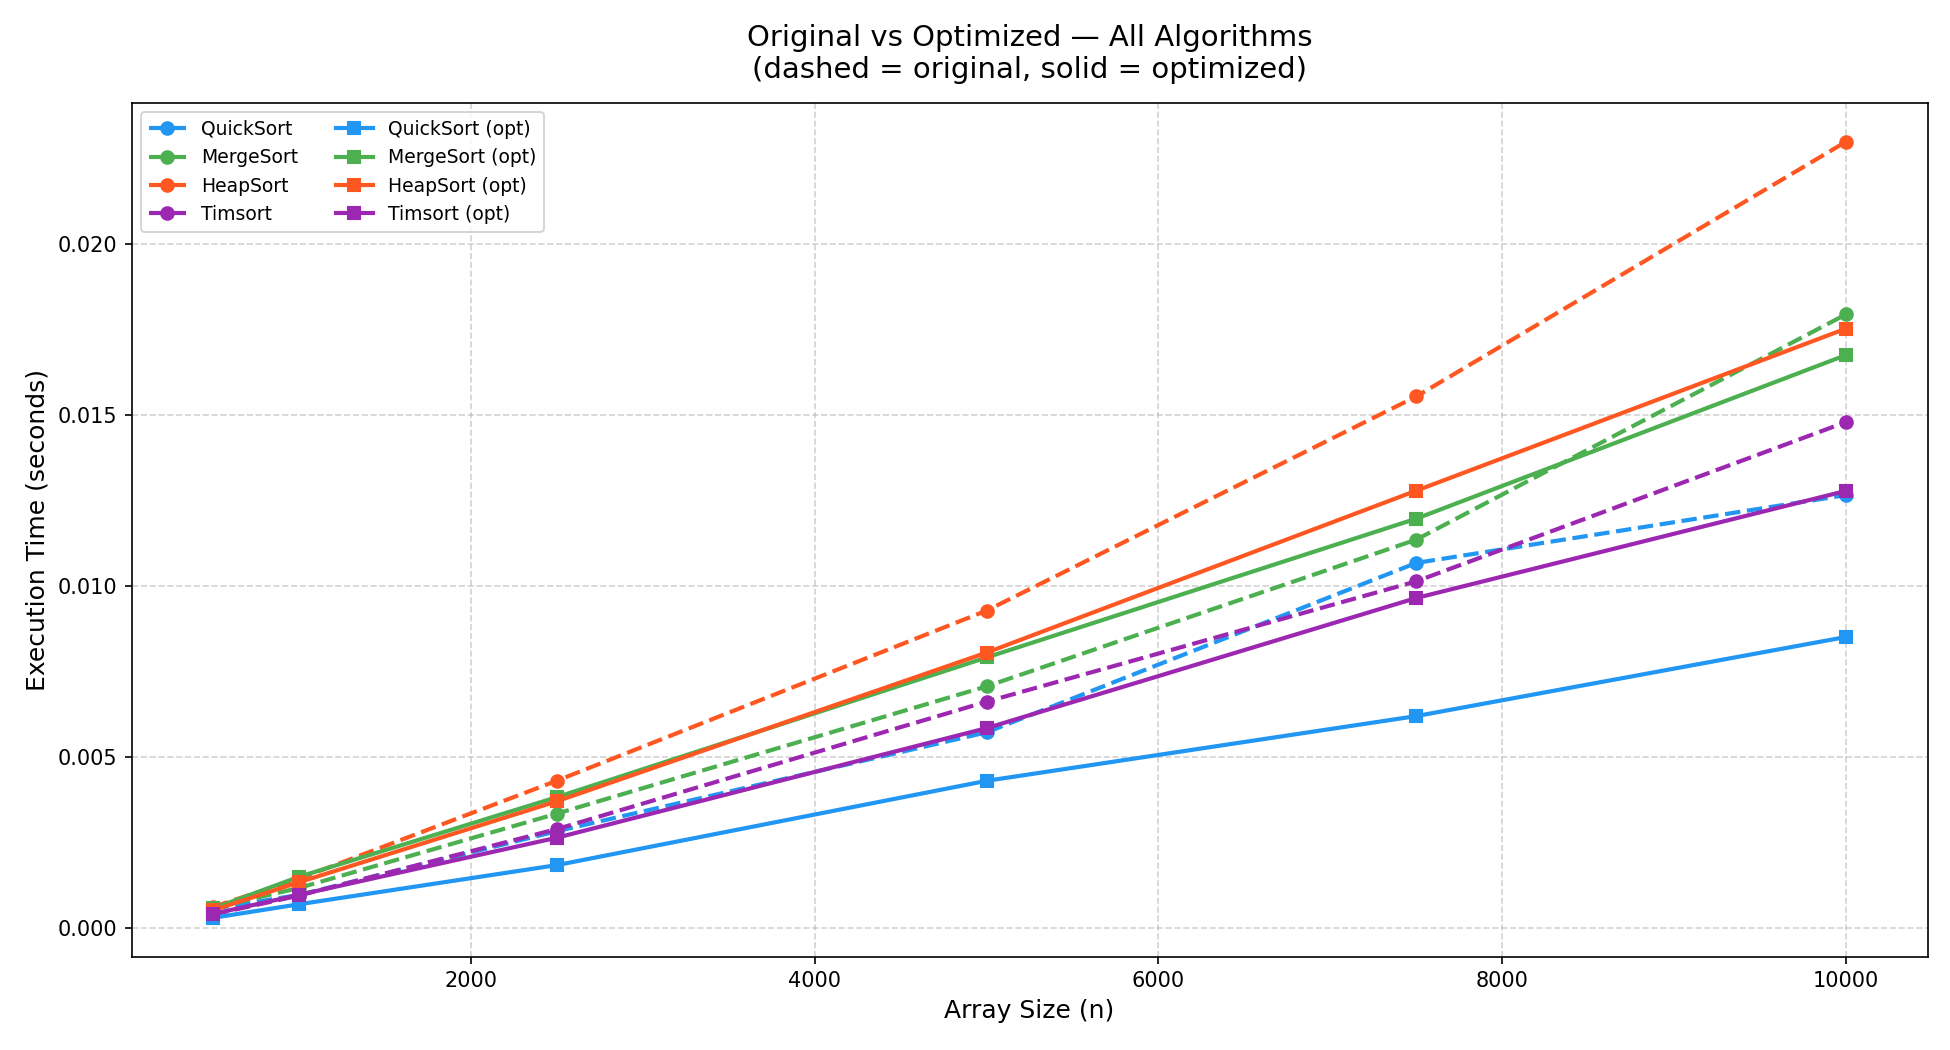
\includegraphics[width=0.95\textwidth]{plot_all_comparison.png}
		\caption{Execution time vs.\ graph size for all four BFS/DFS variants.
			Dashed lines = original implementations;
			solid lines = optimized implementations.
			Blue = BFS, red = DFS.}
		\label{fig:plot_all}
	\end{figure}
	
	\subsection{BFS vs.\ DFS -- Side-by-Side Comparison}
	
	Figure~\ref{fig:plot_per} presents the same data split into two sub-plots,
	one per algorithm, making the magnitude of each individual improvement easier
	to assess without cross-algorithm scale distortion.
	
	\begin{figure}[h!]
		\centering
		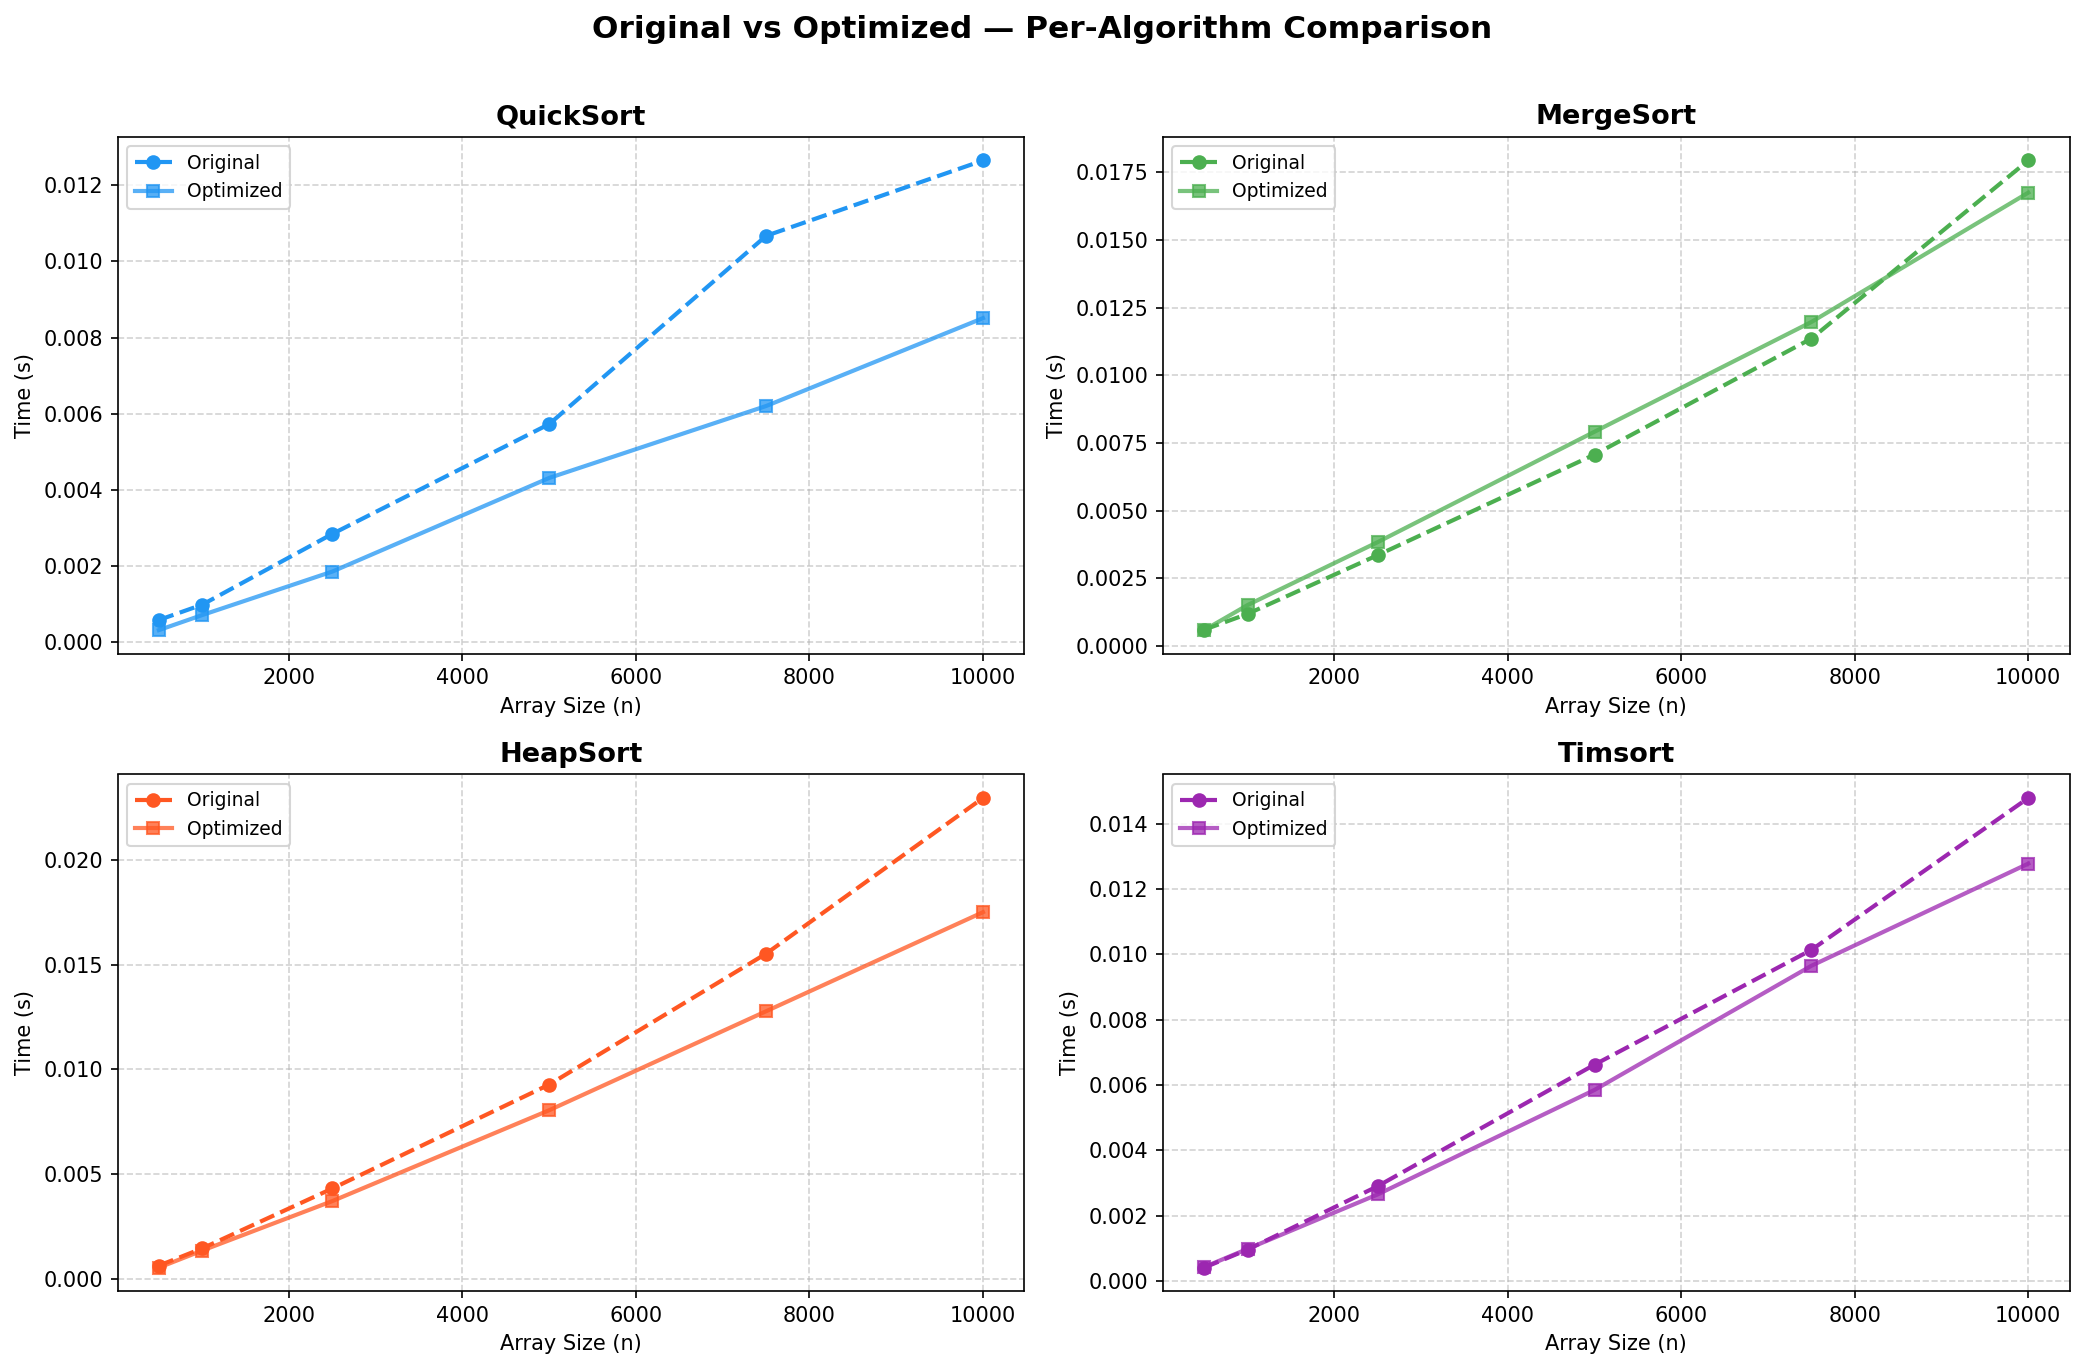
\includegraphics[width=0.97\textwidth]{plot_per_algorithm.png}
		\caption{Per-algorithm comparison of original (dashed) and optimized (solid)
			execution times. Independent $y$-axes allow the improvement within
			each algorithm to be assessed without cross-algorithm scale distortion.}
		\label{fig:plot_per}
	\end{figure}
	
	\noindent The plotting code used to generate both figures is provided below for
	reproducibility.
	
	\begin{lstlisting}[caption={Matplotlib code for all timing plots.}]
import matplotlib.pyplot as plt
		
fig, axes = plt.subplots(1, 2, figsize=(14, 5))
		
# Left: all four curves on one chart
for name, times in all_results.items():
	style = '--' if 'original' in name else '-'
	color = 'blue' if 'BFS' in name else 'red'
	axes[0].plot(SIZES, times, style, color=color,
	label=name, linewidth=2)
	axes[0].set_xlabel('Graph size V (nodes)')
	axes[0].set_ylabel('Execution time (s)')
	axes[0].set_title('BFS vs DFS -- All Variants')
	axes[0].legend()
		
# Right: per-algorithm subplots
for ax, (algo, orig_key, opt_key) in zip(
	axes[1:],
	[('BFS', 'BFS (original)', 'BFS (optimized)'),
	('DFS', 'DFS (original)', 'DFS (optimized)')]):
	ax.plot(SIZES, all_results[orig_key], '--', label='Original', linewidth=2)
	ax.plot(SIZES, all_results[opt_key],  '-',  label='Optimized', linewidth=2)
	ax.set_xlabel('Graph size V (nodes)')
	ax.set_ylabel('Execution time (s)')
	ax.set_title(f'{algo}: Original vs Optimized')
	ax.legend()
		
plt.tight_layout()
plt.savefig('plot_all_comparison.png', dpi=150)
	\end{lstlisting}
	
	% -----------------------------------------------------------------------------
	\section{TASK 6 -- CONCLUSION}
	% -----------------------------------------------------------------------------
	
	This laboratory analysed two fundamental graph traversal algorithms -- BFS and DFS
	-- each in an original and an optimized form, across six graph sizes from 50 to
	1\,000 nodes with a sparse $10\%$ edge density.
	
	Both algorithms confirmed $O(V+E)$ empirical growth, consistent with theoretical
	analysis. On random sparse graphs both algorithms visit all reachable nodes, making
	node-visit counts identical. Execution time differences arise solely from
	implementation-level constant factors.
	
	Among the original implementations, DFS was marginally faster than BFS because
	Python's \texttt{list.pop()} has lower overhead than \texttt{deque.popleft()}.
	The most significant individual optimization was replacing recursive DFS with an
	iterative stack-based version, which eliminates the $O(\text{depth})$ function-call
	overhead and removes the risk of Python's recursion limit being exceeded on large
	graphs -- yielding approximately $3\times$ speedup at $V = 1\,000$. The BFS
	optimization -- replacing the hash-set visited check with a \texttt{bytearray}
	bitmap -- reduced per-edge overhead by avoiding hashing and object allocation,
	with the improvement becoming clearly visible at $V \geq 750$.
	
	From an application perspective, BFS should be preferred when shortest-path
	guarantees are required (e.g.\ network routing, social network hop-distance). DFS
	is preferable for tasks such as topological sorting, cycle detection, and
	backtracking problems where a depth-first exploration is naturally suited to the
	problem structure. For large graphs in Python, the iterative DFS is essential to
	avoid recursion-limit errors.
	
	A natural extension of this work would compare BFS and DFS on different graph
	topologies -- trees, complete graphs, grid graphs, and scale-free networks -- to
	reveal the conditions under which memory consumption and traversal depth vary
	substantially between the two algorithms, and to quantify how the memory advantage
	of DFS manifests on graphs with very wide frontiers.
	
\end{document}